%===============================Bell Trees BT=============================
\documentclass {amsart}
\usepackage[latin1]{inputenc}
\usepackage[dvips]{graphicx}

\newcommand{\emerson}{Emerson A. de O. Lima}
\newcommand{\glaucio}{Glaucio G. de M. Melo}
%=================================Preamble ends here========================================
\begin{document}
\title[Bell Trees]
 {Bell Trees}
%=====================================Title=================================================
\author[Melo]{\glaucio}
\address[Melo]{Departamento de Estat\'{\i}stica e Inform\'{a}tica - UNICAP}
\email[Melo]{glaucio@dei.unicap.br}
%=====================================Melo==================================================
\author[Oliveira-Lima]{\emerson}
\address[Oliveira-Lima]{Departamento de Estat\'{\i}stica e Inform\'{a}tica - UNICAP}
\email[Oliveira-Lima]{eal@dei.unicap.br}
%================================Oliveira Lima==============================================
\keywords{Combinatorial Algorithms, Complexity, Combinatorial
Structures, Partition}
%===================================Key Words===============================================
\begin{abstract}
This article presents a combinatorial structure that only formed
by the Bell Numbers. Is also shown the definition and
demonstration of this structure's properties.
\end{abstract}
%=================================End Abstract=============================================
 \maketitle
%=================================Introduction=============================================
\section*{Introduction}
We can define a Bell Number as a number of partitions possibilities of a
set with {$n$} elements. Such number is defined by:

\begin{equation} \label{eq1}
B_n = \sum_{k=1}^{n} \bigg\{{n\atop k}\bigg\}
\end{equation}

Where {$\big\{{n\atop k}\big\}$} is the Stirling number of second
kind, which is defined by:

\begin{equation} \label{eq2}
\bigg\{{n\atop k}\bigg\} = \frac{1}{k!} \sum_{i=0}^{k-1}(-1)^i {k
\choose i}(k-i)^n
\end{equation}


With the definitions \ref{eq1} and \ref{eq2} above, this article
proposes to show a combinatorial structure which is called here
\emph{Bell Tree} and the use of this structure to solve the
\emph{Partition of an n-Set} problem. It was used as basis the
definition of a partition tree, shown in the algorithm \emph{Next
Partition of an n-Set}\cite{wi}, associating the tree nodes with
the equations which its terms are defined on the tree construction
properties.


\section*{Properties of Bell Trees}

Let {$n$} be the number of elements of a set that will be
partitioned and {$B$} the Bell Numbers that denotes a set of terms
that can form a mathematical expression in a node of the tree, the
structure here defined adopt the partition tree structure with
{$n$}-Sets and added to it others properties. Follows below some
properties of the structure:

\begin{itemize}

\item The Tree has {$n$} levels;

\item The Tree nodes are non-negative integers numbers which is
formed by expressions that evolves exclusively Bell Numbers and
multiplicative integer constants;

\item Let {$S$} be a subset contained in {$B$} which denotes the
number of distinct terms of an expression with a node {$N$}, we
determine the number of descendants produced by {$N$} from the
number of elements of {$S$} increased one unit;

\item The number {$R$} of the nodes on a Bell Tree corresponds to:

\begin{equation} \label{eq3}
R = \sum_{j=1}^{n}B_j
\end{equation}

\item Let {$k$} be the number of descendants of the actual node
{$N$}, the value for all its {$k-1$} are defined by:

Let {$E_w$} be a mathematical expression with {$w$} terms from the
ascendant node, the descendant node corresponds to {$E_{w-1}$}.
To illustrate such fact, if we have a ascendant node represented
by the expression:

\begin{equation} \label{eq4}
E_w = (B_w - B_{w-1}) - 2(B_{w-1} - B_{w-2})
\end{equation}
Then, the descendants nodes will correspond to the expression:

\begin{equation} \label{eq5}
E_{w-1} = (B_{w-1} - B_{w-2}) - 2(B_{w-2} - B_{w-3})
\end{equation}
For the {$k$}-tuple descendant of {$N$}, we have the expression:

\begin{equation} \label{eq6}
E_k = E_w - (k-1)E_{w-1}
\end{equation}
That it is equivalent to say that the {$k$}-tuple descendant is
equal to the ascendant node value minus {$k-1$} times the value of
the others descendant nodes.

\end{itemize}

We can now make a tree that follows this formation law. For {$n = 5$},
we have a tree illustrated on Figure \ref{a1}. The three first levels
expressions of this tree are in Table \ref{t1}, which the number of nodes
are entered from top to bottom and from left to right.

\begin{table}[!hbp]
  \caption{Nodes values of the Tree illustrated on Figure \ref{a1}}
  \label{t1}
\begin{tabular}{l|l}
 \hline
   Nodes  & Expressions  \\
 \hline
    1   & {$B_5$}\\
  \hline
    2   & {$B_4$}\\
  \hline
    3   & {$B_5 - B_4$}\\
  \hline
    4   & {$B_3$}\\
  \hline
    5   & {$B_4 - B_3$}\\
  \hline
    6   & {$B_4 - B_3$}\\
  \hline
    7   & {$B_4 - B_3$}\\
  \hline
    8   & {$(B_5 - B_4) - 2(B_4 - B_3$)}\\
 \end{tabular}
\end{table}

\begin{figure}
  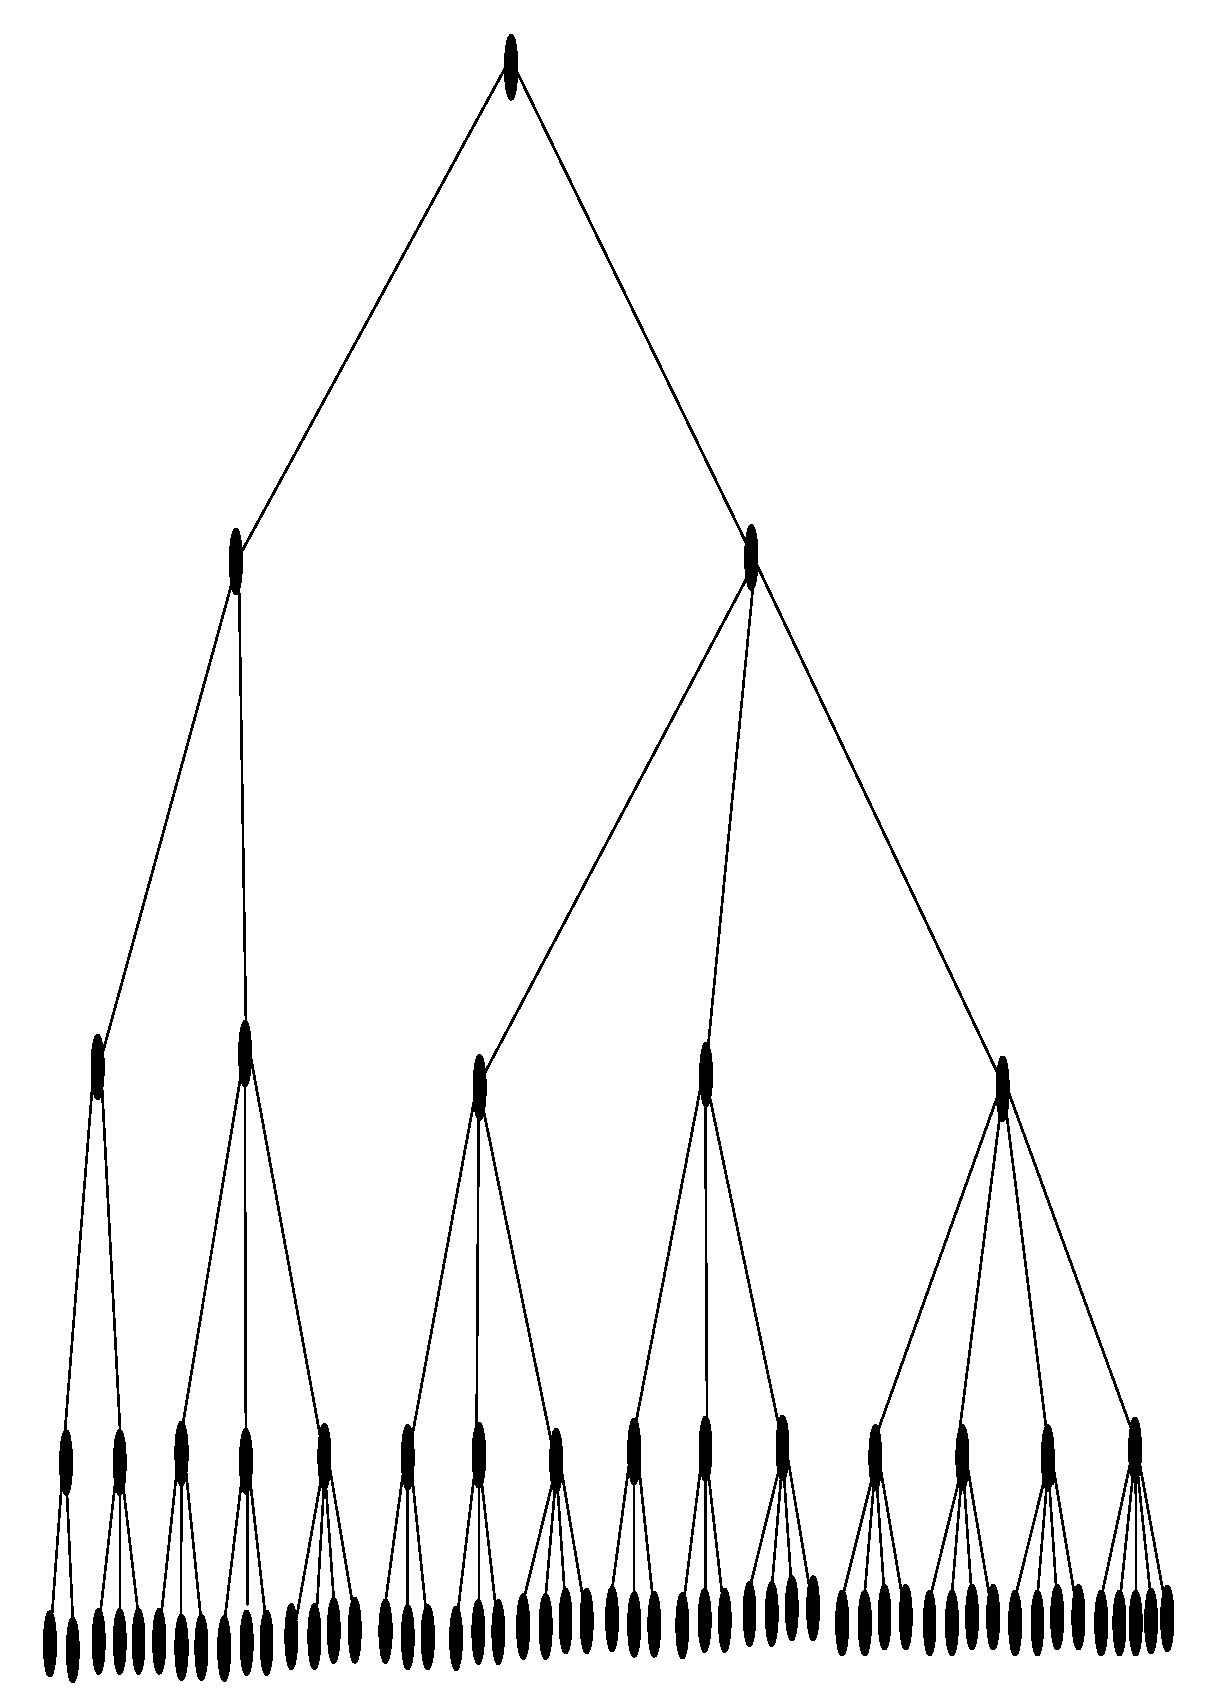
\includegraphics[width=290pt,height=80pt]{BT5}
  \caption{Bell Tree with level 5}\label{a1}
\end{figure}

\section*{Search Analysis and Verification of  Serials on Bell Tree}

The Bell Tree stands the search of serial numbers placed between
{$1$} and {$B_n$}. A typical search algorithm does {$n$}
interactions on the number of levels that the tree can goes deep
in maximum {$k-1$} interactions inside of each tree level, where
{$k$} represents the number of descendants of the visited node.
This algorithm works on {$O(nk)$} in the worst case. The use of
search algorithms and serial numbers verification on this
combinatorial structure is related to the production of the subset
indexes partitioned from a set of {$n$} elements, giving as an
input its position on the list of partitions\cite{me}. Such set of
indexes can be represented by vector {$p$} with size {$n$}. On
each current level of the tree, the nodes are enumerated from zero
and from left to right and each {$p$} component receives the value
referring to the last index visited on each level of the Bell
Tree.

\section*{Demonstration}
(This section is not ready)

%===========================BIBLIOGRAFIA==============================================
\begin{thebibliography}{99}
\bibitem{wi} WILF, Herbert S., NIJENHUIS, A. ~Combinatorial Algorithms for computers and calculators. Academic
Press, INC, 1978.
\bibitem{me} MELO, Glaucio G. de M., OLIVEIRA-LIMA, Emerson A. de O. Serial Partition of an n-Set Method,
(Not published yet),2004.
\end{thebibliography}
\end{document}
